\begin{circuitikz}[background rectangle/.style={fill=white}, show background rectangle]
    \node(0,0) {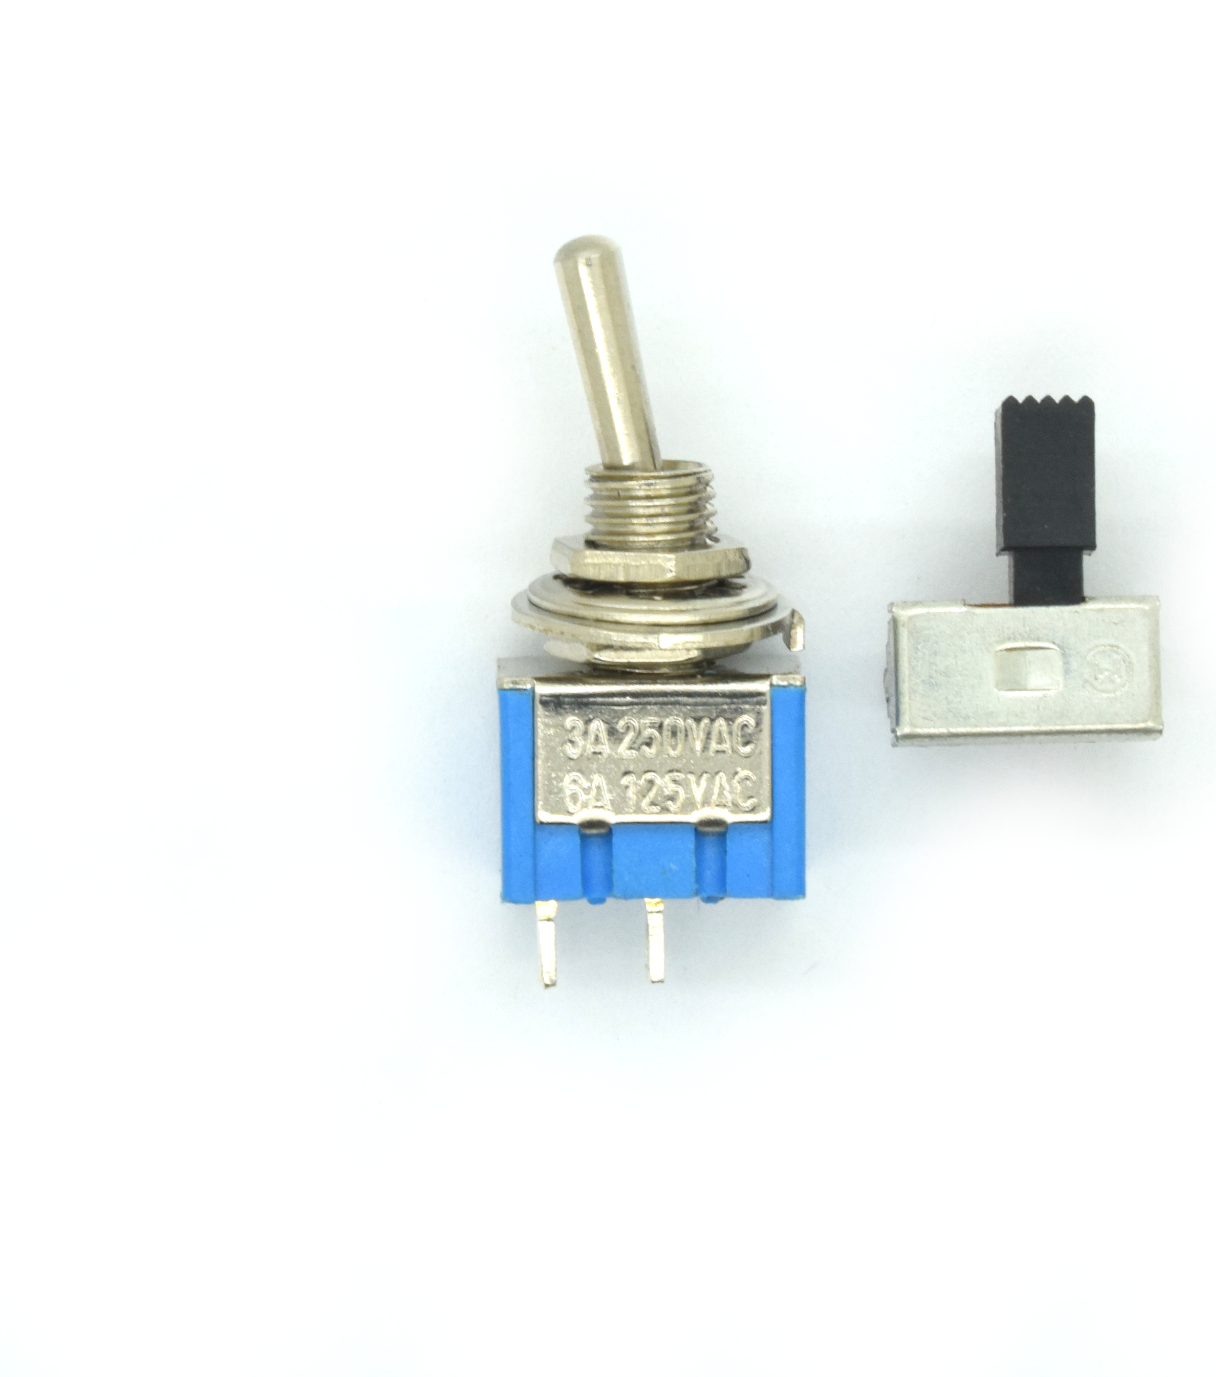
\includegraphics[width=200pt]{foto/5}};
    
    %Schalter Offen:
    \draw(-1.5,-2.5)
    to [short, -*] ++(0.5,0) coordinate(foo)
    to [open] ++(1,0)
    to [short, *-] ++(0.5,0) coordinate(c1);
    \draw[thick] (foo) to [short] ++(1,0.0); % Closed
    \draw(c1) node[right=0.0] {\small Geschlossen};
    
    %Schalter Offen:
    \draw(-1.5,-3.5)
    to [short, -*] ++(0.5,0) coordinate(foo)
    to [open] ++(1,0)
    to [short, *-] ++(0.5,0) coordinate(c2);
    \draw[thick] (foo) to [short] ++(1,0.5); % Open
    \draw(c2) node[right=0.0] {\small Offen};

    % Beschriftung:
    \draw( 2.25, 2.25) node {\small Schiebeschalter};
    \draw( 0.25, 3.00) node {\small Kippschalter};

    % Pfeile:
    \draw[>=triangle 60, <->] (-2.25,0.675) coordinate(c1) -- ++(0,-1.35) coordinate(c2);
    \draw(c1) -- ++( 0.25,0);
    \draw(c1) -- ++(-0.25,0);
    \draw(c2) -- ++( 0.25,0);
    \draw(c2) -- ++(-0.25,0);

    % Text:
    \draw (c1) ++ (0,0.25) node {\qty{1}{\centi\meter}};
\end{circuitikz}